\documentclass[10pt]{beamer}

%\usetheme{ENSLyon}

\usetheme{AnnArbor}

\title[Libras II]{\Large \textsc{Escrita de Sinais}}
\author[G. Philippi]{{Guilherme Philippi\vspace{-0.3cm}}}
\institute[]{Departamento de Matemática\\ Universidade Federal de Santa Catarina, Blumenau \\ \vspace{0.2cm} Professora orientadora Fabiana Schmitt Corrêa\vspace{-0.2cm}}
\date[15 Março, 2022]{{\small Libras II}\\{\scriptsize Seminário\\ 15 de Março de 2022}}
\setbeamersize{text margin left=5mm}
\setbeamersize{text margin right=5mm}

\setbeamertemplate{navigation symbols}{}
%\usecolortheme{ENSLyon_greener}
\usecolortheme{whale}

\setbeamercolor{frametitle}{bg=gray}
\setbeamertemplate{bibliography item}{\insertbiblabel}

%PACKAGES -------------------------
\usepackage{etex}
\usepackage[utf8]{inputenc}
\usepackage[brazilian]{babel}
\usepackage{enumerate}
\usepackage{amsmath}
\usepackage{amssymb}
\usepackage{amsthm}
\usepackage{amscd}
\usepackage{amsfonts}
\usepackage{multicol}
\usepackage{multirow}
\usepackage{array}
\usepackage{color}
\usepackage{graphicx}
\usepackage{tikz}
\usepackage{tikz-qtree}
\usepackage{wrapfig}
\usepackage{3dplot}
\usepackage{pgf}
\usepackage{tkz-euclide}
\usepackage{algorithmic}
\usepackage{algorithm}
\usepackage{xparse}
\usepackage{subfigure}

%LIBRARIES-TIKZ ------------------------------------------

\usetikzlibrary{shadows,trees}
\usetikzlibrary{decorations.pathmorphing}
\usetikzlibrary{decorations.markings}
\usetikzlibrary{positioning}
\usetikzlibrary{chains,matrix,scopes}
\usetikzlibrary{arrows}

%DEFINITIONS ----------------------------------------------------

\def\centerarc[#1](#2)(#3:#4:#5)% Syntax: [draw options] (center) (initial angle:final angle:radius)
{ \draw[#1] ($(#2)+({#5*cos(#3)},{#5*sin(#3)})$) arc(#3:#4:#5); }
\def\xx{\mathbf{x}}
\def\ii{\mathbf{i}}
\def\jj{\mathbf{j}}
\def\kk{\mathbf{k}}
\def\tt{\mathbf{t}}
\def\ee{\mathbf{e}}
\def\qq{\mathbf{q}}
\def\pp{\mathbf{p}}
\def\vv{\mathbf{v}}
\def\rr{\mathbf{r}}
\def\vzero{\mathbf{0}}
\def\qset{\mathbb{H}}
\def\xx{\mathbf{x}}


\AtBeginSection[]
{
	\begin{frame}<beamer>
		\frametitle{Inicio da seção \thesection}
		\tableofcontents[currentsection]
	\end{frame}
}


%NEW THEOREMS ------------------------------------------

\theoremstyle{plain}
\newtheorem{teorema}{Teorema}[section]
\newtheorem{lema}{Lema}[section]
\newtheorem{proposicao}{Proposição}[section]
\newtheorem{corolario}{Corolário}[section]

\theoremstyle{definition}
\newtheorem{definicao}{Definição}[section]
\newtheorem{observacao}{Observação}[section]
\newtheorem{exemplo}{Exemplo}[section]

\newenvironment{solucao}
{\renewcommand\qedsymbol{$\triangle$}\begin{proof}[Solução]}{\end{proof}}



\begin{document}
	
	%FACE
	\begin{frame}
		
		\titlepage
		
		\vspace{-0.6cm}
		\begin{flushleft}
			
\includegraphics[scale=0.15]{logo.png}
		\end{flushleft}
		
		\vspace{-2.2cm}
		\begin{flushright}
			
\includegraphics[scale=0.024]{logo_ufsc.png}
		\end{flushright}
	\end{frame}
	
	%Indice
	\begin{frame}
		\tableofcontents 
	\end{frame}
	
	\section{Contexto histórico}
	
	\begin{frame}
		\frametitle{Surgimento} 
		{
			A \textbf{Escrita de Sinais} (originalmente, \textbf{\textit{SignWriting}}) foi criada em 1974 pela dançarina norte americana \textbf{Valerie Sutton}. Inicialmente, o objeto de Sutton era desenvolver uma forma de registro para a dança, o que originou a \textit{DanceWriting}.
			
			\vspace{0.5cm}
			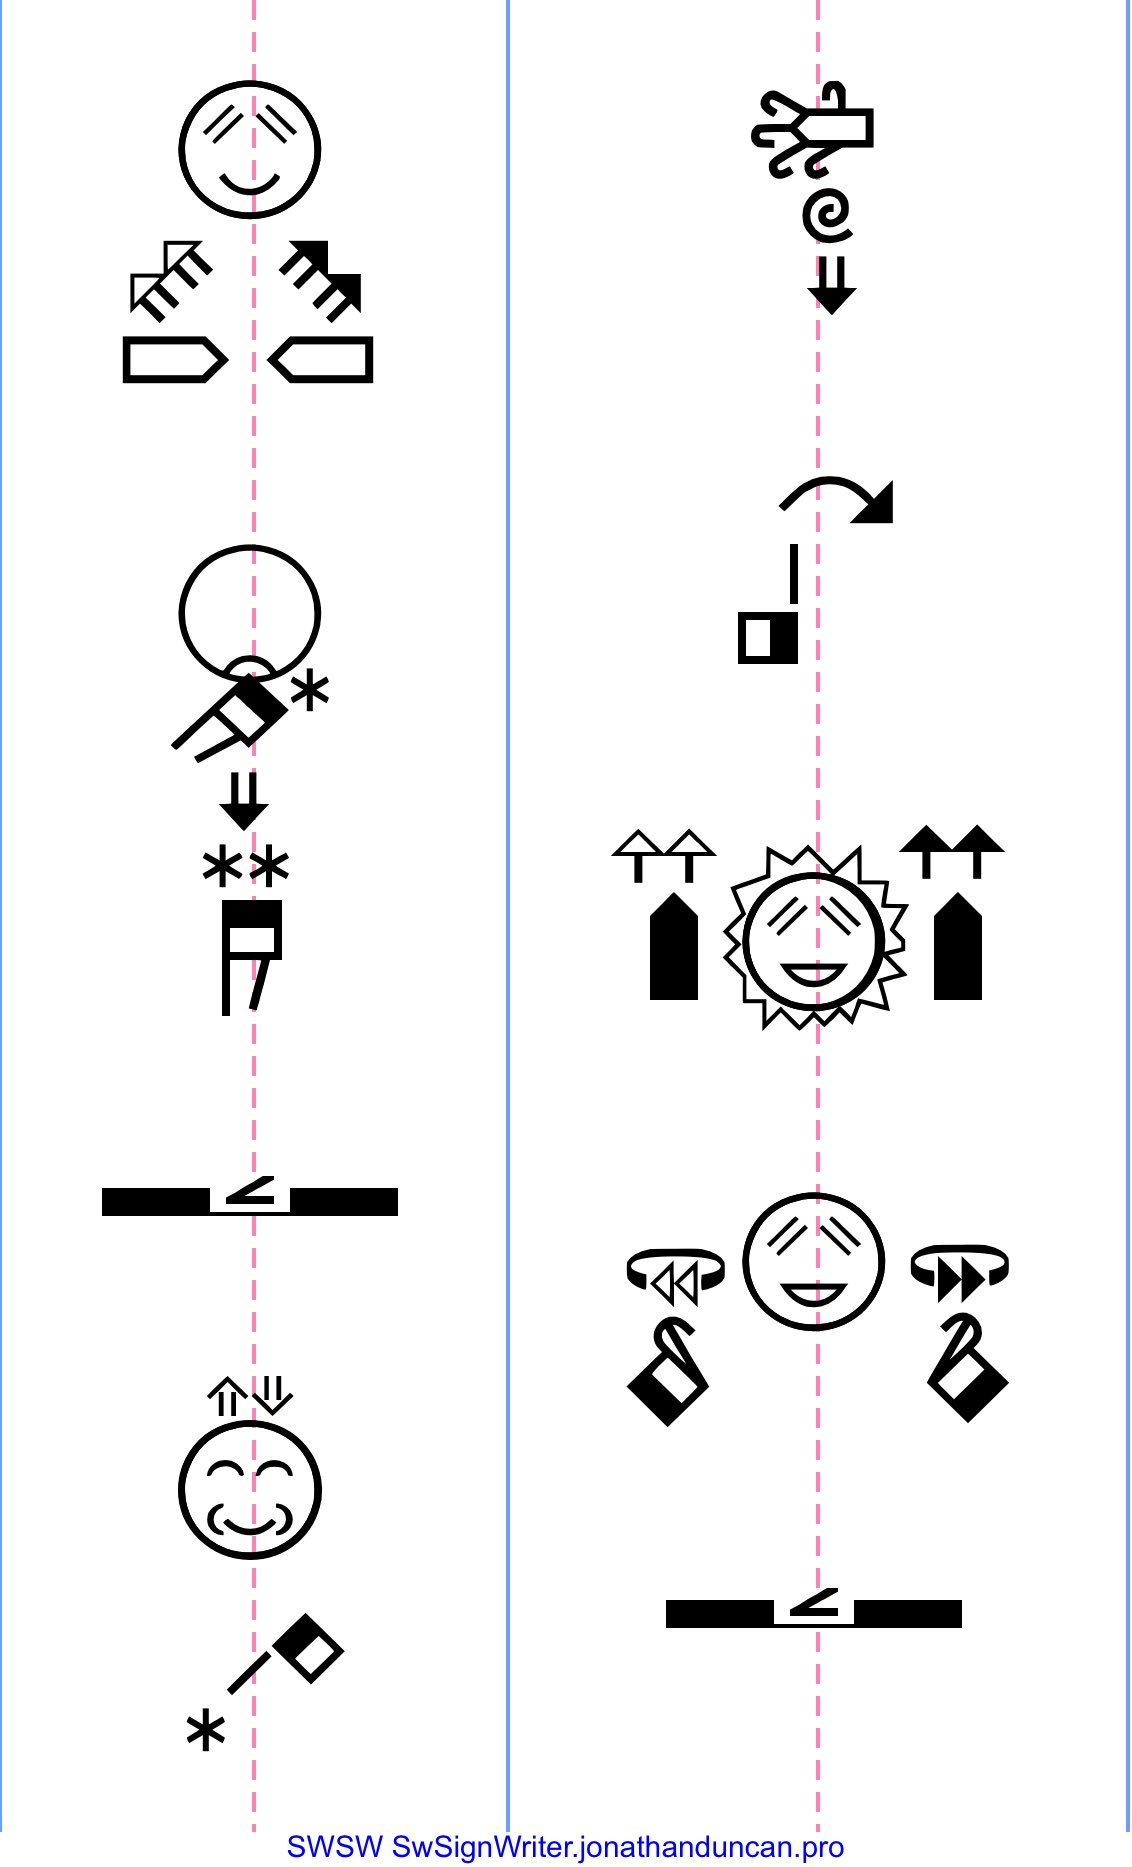
\includegraphics[scale=0.06]{figures/5ed8f275ad7ce03f8e6c80ac20281566.jpg}
			
			\vspace{-4.0cm}
			\hspace{3cm}
			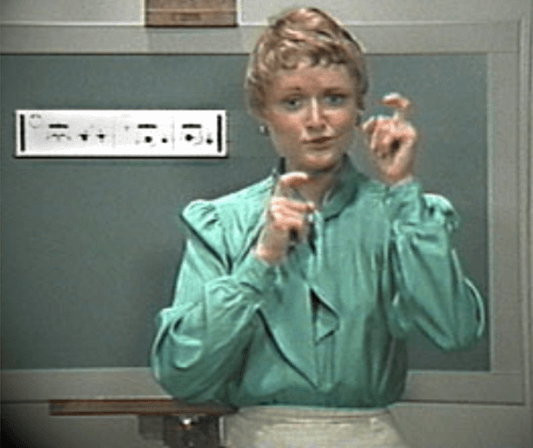
\includegraphics[scale=0.2]{figures/valerie-sutton-ensinando-signwriting-1985.png}
			
			{\vspace{-3.0cm}
				\hspace{6.8cm}
			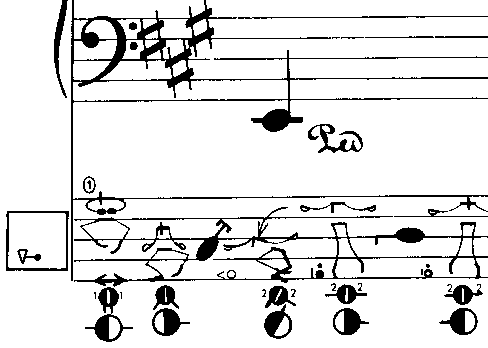
\includegraphics[scale=0.26]{figures/dwd0040.png}
			}
		
			\vspace{1.0cm}
			Além destes, Sutton também desenvolveu os sistemas \textit{MimeWriting}, \textit{SportsWriting}, \textit{ScienceWriting} \cite{sutton2015history}.
		}	
	\end{frame}

	\begin{frame}
		\frametitle{Utilização}
		
		Já são \textbf{mais de 35 países que utilizam esse sistema} de escrita em escolas, universidades, associações e demais áreas ligadas à comunidade surda.
		\vspace{0.5cm}
		
		Como essa forma de escrita \textbf{representa os movimentos da Língua de Sinais}, ela pode ser utilizada para qualquer uma, \textbf{independente de localidade}.
		
		\begin{center}
			\begin{minipage}{0.3\linewidth}
				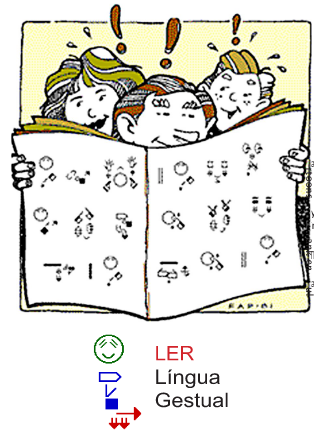
\includegraphics[scale=0.24]{figures/ler.png}
			\end{minipage}
			\begin{minipage}{0.3\linewidth}
				
\includegraphics[scale=0.24]{figures/escrever.png}
			\end{minipage}
			\begin{minipage}{0.3\linewidth}
				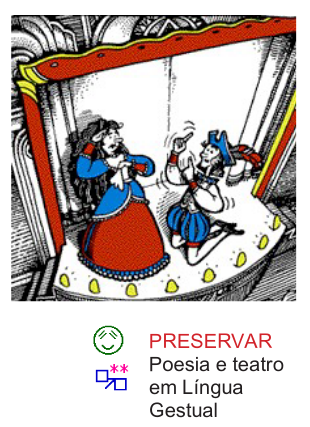
\includegraphics[scale=0.24]{figures/preservar.png}
			\end{minipage}
		\end{center}
	\end{frame}

	\begin{frame}
		\frametitle{Digitalização do método}
		
		Já existem \textbf{softwares} para a escrita de sinais \cite{rocha2001signwriting}. Assim, é possível \textbf{traduzir textos} para a escrita de sinais, de forma que a \textbf{leitura} para os utilizadores de Língua dos Sinais é dada de \textbf{forma natural}.
		
		\begin{center}
			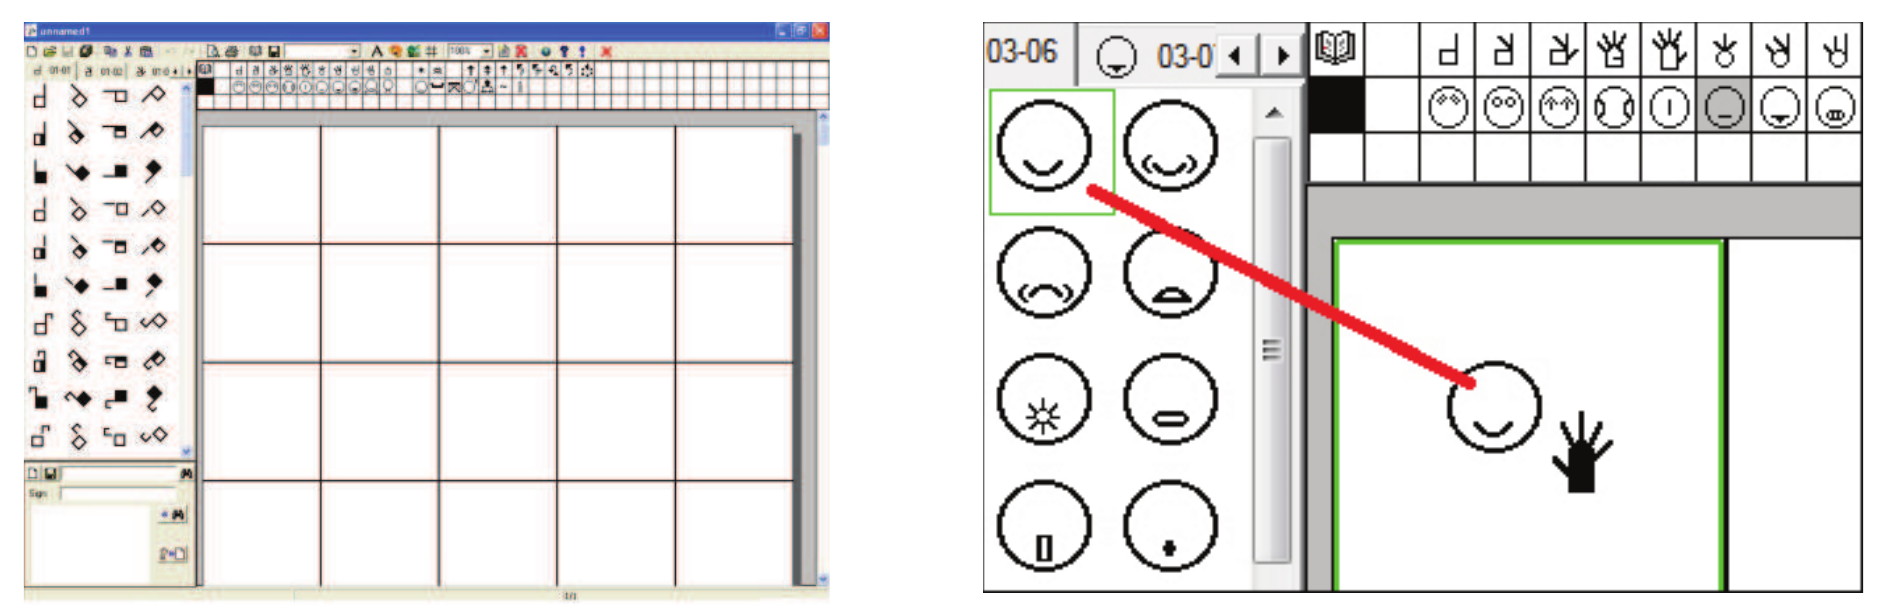
\includegraphics[scale=0.24]{figures/software.png}
		\end{center}
	\end{frame}
	
	\section{Estrutura básica}
	
	\begin{frame}
		\frametitle{Estrutura básica da escrita de sinais}
		\begin{center}
			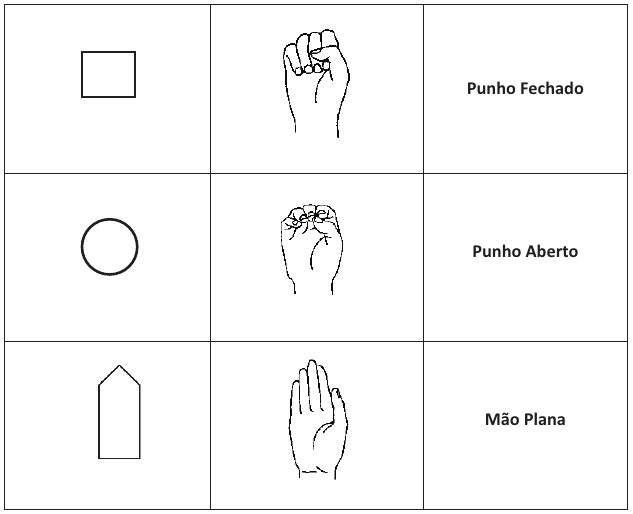
\includegraphics[scale=0.54]{figures/basico.png}
		\end{center}
	\end{frame}

	\begin{frame}
		\frametitle{Estrutura básica da escrita de sinais}
		\begin{center}
			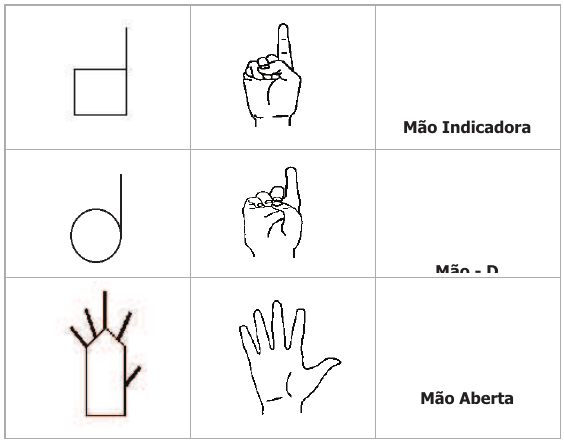
\includegraphics[scale=0.54]{figures/basico2.png}
		\end{center}
	\end{frame}

	\begin{frame}
		\frametitle{Estrutura básica da escrita de sinais}
		\begin{center}
			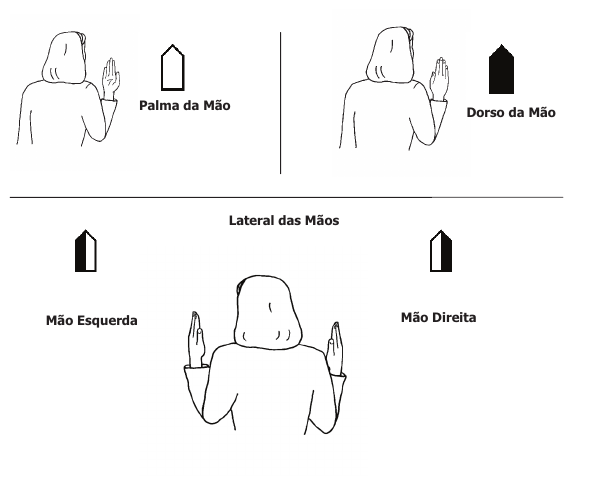
\includegraphics[scale=0.54]{figures/basico3.png}
		\end{center}
	\end{frame}

	\begin{frame}
		\frametitle{Estrutura básica da escrita de sinais}
		\begin{center}
			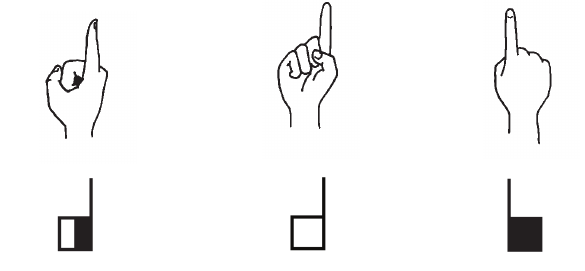
\includegraphics[scale=0.54]{figures/basico3-1.png}
		\end{center}
	\end{frame}

	
	\begin{frame}
		\frametitle{Estrutura básica da escrita de sinais}
		\begin{center}
			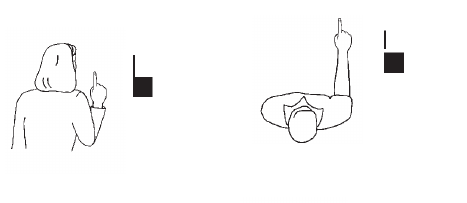
\includegraphics[scale=0.54]{figures/basico4.png}
			
			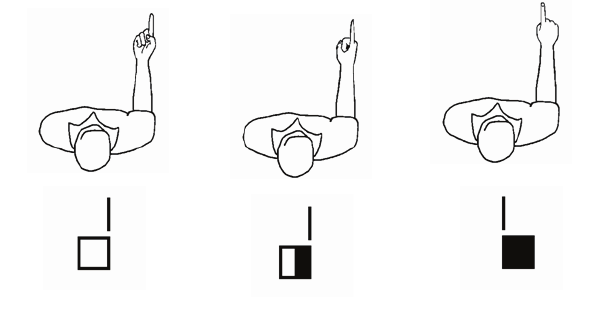
\includegraphics[scale=0.54]{figures/basico4-1.png}
		\end{center}
	\end{frame}

	
	\begin{frame}
		\frametitle{Estrutura básica da escrita de sinais}
		\begin{center}
			Movimento com mão esquerda: Seta branca
			
			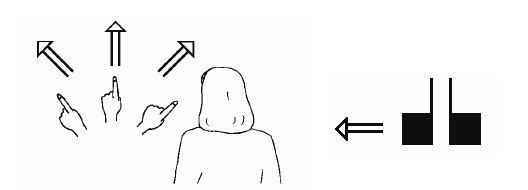
\includegraphics[scale=0.54]{figures/basico5.png}
			\vspace{0.5cm}
			
			
			Movimento com mão direita: Seta preta
			
			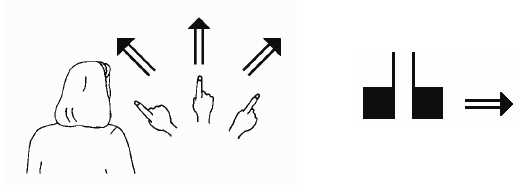
\includegraphics[scale=0.54]{figures/basico5-1.png}
		\end{center}
	\end{frame}
	
	\begin{frame}
		\frametitle{Estrutura básica da escrita de sinais}
		\begin{center}
			\begin{minipage}{0.3\linewidth}
				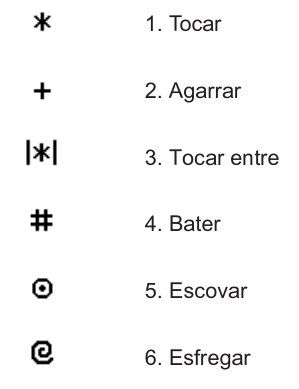
\includegraphics[scale=0.34]{figures/basico6.png}
			\end{minipage}
			\hspace{1cm}
			\begin{minipage}{0.3\linewidth}
				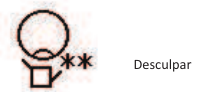
\includegraphics[scale=0.54]{figures/basico6-1.png}
				\vspace{0.2cm}
				
				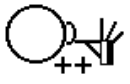
\includegraphics[scale=0.4]{figures/basico6-2.png} Brinco
				\vspace{0.2cm}
				
				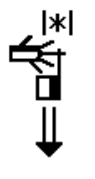
\includegraphics[scale=0.4]{figures/basico6-3.png} Desaparecer
				\vspace{0.2cm}
				
				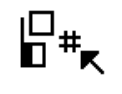
\includegraphics[scale=0.4]{figures/basico6-4.png} Bater
			\end{minipage}
			\hspace{0.5cm}
			\begin{minipage}{0.2\linewidth}
				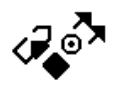
\includegraphics[scale=0.4]{figures/basico6-5.png} 
				
				Escovar
				\vspace{0.5cm}
				
				
\includegraphics[scale=0.4]{figures/basico6-6.png} 
				
				Café				
			\end{minipage}
			
		\end{center}
	\end{frame}

		\begin{frame}
			\frametitle{Alfabeto em escrita de sinais}
			\begin{center}
				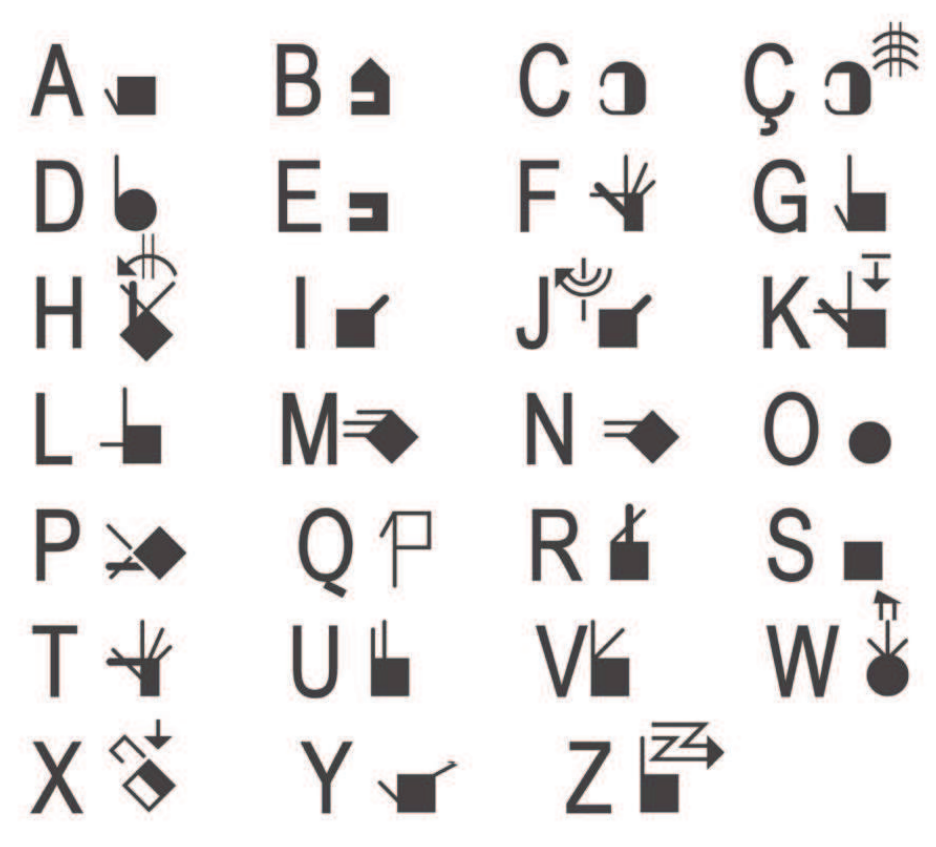
\includegraphics[scale=0.3]{figures/alfabeto.png}
			\end{center}
		\end{frame}
	
	
	\section{Referências}
	%Slide refe
	\begin{frame}		
		
		{\footnotesize
		\bibliographystyle{unsrt}
		\bibliography{references}}
	\end{frame}
	
	%Slide End
	\begin{frame}
		\begin{center}
			\vspace{1.5cm}
			Obrigado!\\
			\hspace{-4.5cm}
			
\includegraphics[scale=0.2]{logo.png}
			
			\vspace{-2.7cm}
			\hspace{5.5cm}
			
\includegraphics[scale=0.038]{logo_ufsc.png}
			
			\vspace{0.5cm}
			Contato: g.philippi@grad.ufsc.br\\ UFSC - Blumenau
		\end{center}
	\end{frame}
	
\end{document}